\chapter{Charakterystyka wykorzystanych komponentów sprzętowych}
    \section{Mikrokontroler Arduino Uno}

    \begin{figure}[h!]
        \centering
        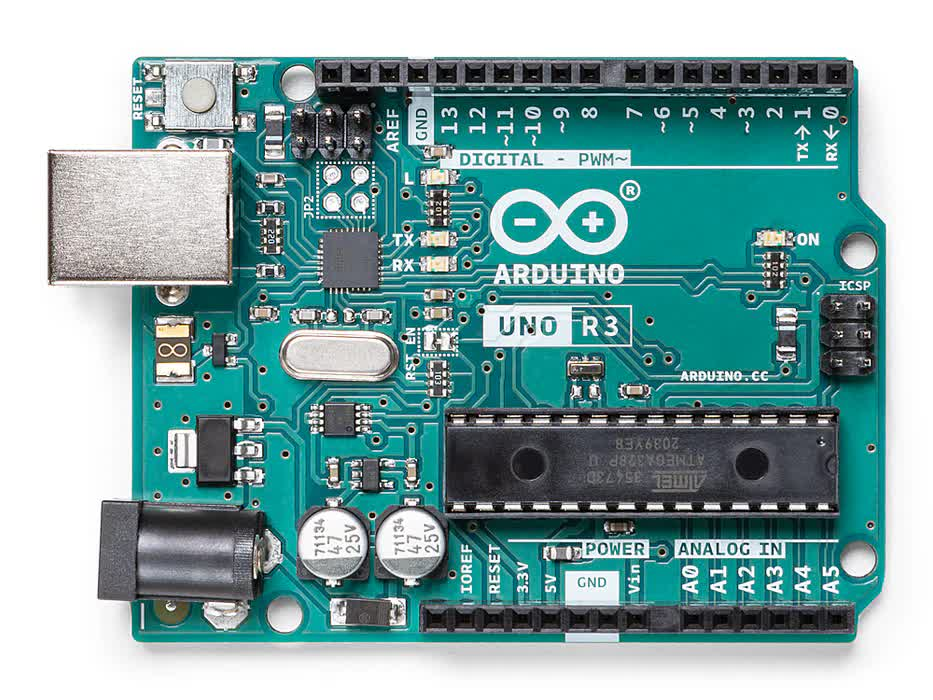
\includegraphics[width=0.35\textwidth]{images/uno.jpg}
        %\caption{Podpis pod obrazkiem.}
        \label{fig:example}
    \end{figure}

    Arduino Uno to popularny mikrokontroler wykorzystywany w projektach elektronicznych i robotyce. Jest to wszechstronna platforma programistyczna oparta na mikrokontrolerze ATmega328P. Mikrokontroler ten posiada 32KB pamięci Flash, 2KB pamięci RAM, 14 cyfrowych pinów wejścia/wyjścia, 6 pinów wejścia analogowego, zegar taktowany z częstotliwością 16MHz, interfejs USB, złącze zasilania 5V oraz złącze programowania ISP. Arduino Uno jest kompatybilny z wieloma dodatkowymi modułami, co pozwala na rozbudowę funkcjonalności. Mikrokontroler ten jest wykorzystywany w projekcie jako główny kontroler systemu.

    \vspace{12pt}

    Programowanie Arduino Uno odbywa się w dedykowanym środowisku Arduino IDE, które wykorzystuje język bazujący na C++. Dzięki rozbudowanej bibliotece funkcji i dużej społeczności użytkowników, realizacja nawet zaawansowanych projektów jest stosunkowo prosta \cite{4}
    
    \section{Czujnik temperatury MLX90614}

    \begin{figure}[h!]
        \centering
        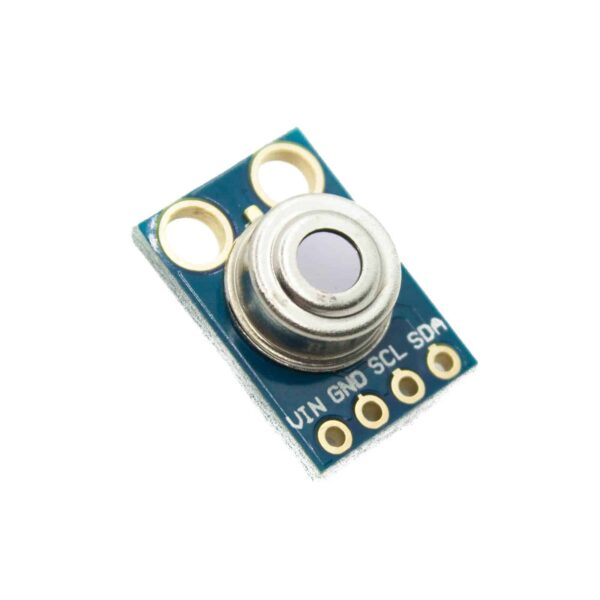
\includegraphics[width=0.35\textwidth]{images/mlx.jpg}
        %\caption{Podpis pod obrazkiem.}
        \label{fig:example}
    \end{figure}

    Czujnik MLX90614 to zaawansowany, bezdotykowy termometr na podczerwień, który umożliwia pomiar temperatury obiektów w szerokim zakresie. Działa na napięciu zasilania od 3V do 3.6V i komunikuje się za pomocą interfejsu I2C, co czyni go łatwym w integracji z różnymi systemami, takimi jak Arduino czy inne mikrokontrolery. Dzięki swojej konstrukcji, MLX90614 znajduje zastosowanie w wielu dziedzinach, w tym w medycynie do pomiaru temperatury ciała, w systemach klimatyzacji oraz w automatyzacji przemysłowej \cite{5}.

    \section{4-przyciskowa klawiatura}

    \begin{figure}[h!]
        \centering
        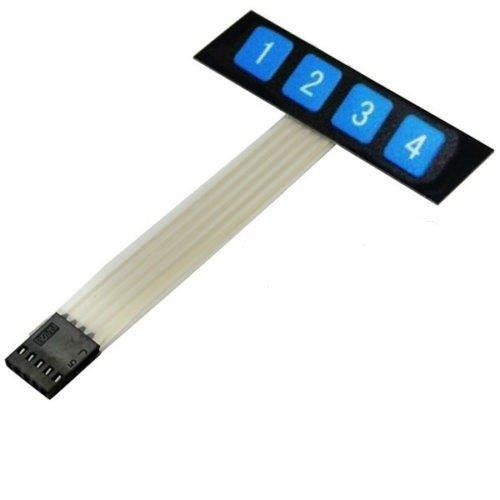
\includegraphics[width=0.35\textwidth]{images/keyboard4pin.jpg}
        %\caption{Podpis pod obrazkiem.}
        \label{fig:example}
    \end{figure}

    Pokazana na zdjęciu klawiatura to membranowa klawiatura numeryczna, składająca się z czterech przycisków oznaczonych cyframi od 1 do 4. Charakteryzuje się prostą budową, elastyczną taśmą zakończoną złączem z pinami, co umożliwia łatwe podłączenie do mikrokontrolera lub innych urządzeń elektronicznych. Tego typu klawiatury są często wykorzystywane w prostych projektach elektronicznych, takich jak panele sterujące, systemy wprowadzania kodów czy interfejsy użytkownika w urządzeniach DIY. Dzięki niskiej cenie i kompaktowym rozmiarom, są popularnym wyborem wśród hobbystów i studentów elektroniki.

    \section{Wyświetlacz LCD z konwerterem I2C HD44780}

    \begin{figure}[h!]
        \centering
        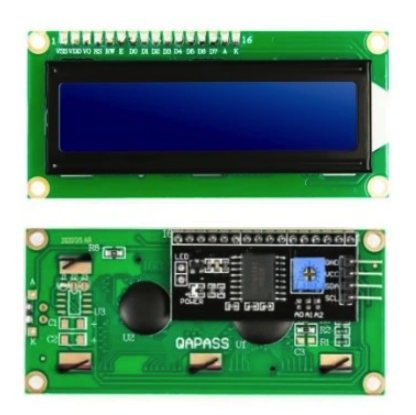
\includegraphics[width=0.3\textwidth]{images/lcd.png}
        %\caption{Podpis pod obrazkiem.}
        \label{fig:example}
    \end{figure}
    
    Wyświetlacz LCD z konwerterem I2C oparty na sterowniku HD44780 to popularne rozwiązanie do wyświetlania tekstu w projektach elektronicznych. Dzięki wbudowanemu konwerterowi I2C znacznie uproszczona jest komunikacja z mikrokontrolerem, ponieważ wymaga jedynie dwóch linii sygnałowych (SDA i SCL), zamiast standardowych 6-8 w przypadku klasycznego podłączenia. Wyświetlacz obsługuje różne konfiguracje, najczęściej spotykane to 16x2 (16 znaków na 2 liniach) lub 20x4 (20 znaków na 4 liniach). Sterownik HD44780 umożliwia łatwe sterowanie wyświetlanymi znakami oraz tworzenie niestandardowych symboli. Dzięki czytelnemu interfejsowi i szerokiemu wsparciu w bibliotekach do Arduino, Raspberry Pi i innych platform, wyświetlacz ten jest chętnie używany w projektach takich jak panele kontrolne, wskaźniki statusu czy urządzenia IoT.